\chapter{Protocolo experimental}\label{cap:protocolo}

\section{Unidade experimental e proveniência}

A cena \textit{study} é a unidade experimental. Ela representa um ambiente de trabalho com mesas, cadeiras, armário e objetos menores sobre o mobiliário. A Figura~\ref{fig:study_scene} apresenta uma vista RGB do próprio DM-SR, diferente das quatro vistas usadas posteriormente na comparação quantitativa. Essa imagem permite reconhecer os elementos cuja aparência, geometria e separação são avaliadas ao longo do protocolo.

\begin{figure}[H]
  \centering
  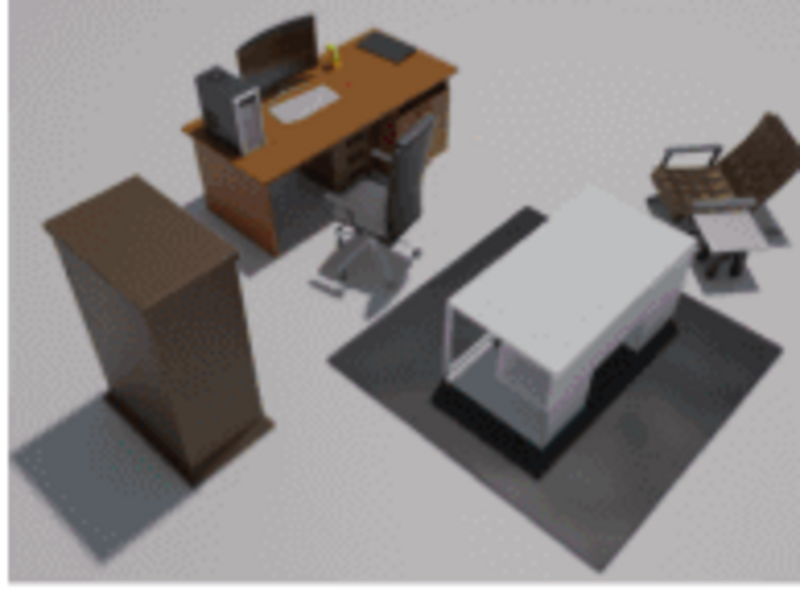
\includegraphics[width=0.60\textwidth]{study_scene_reference.png}
  \caption{Vista RGB de referência da cena \textit{study}, usada como estudo de caso. A cena contém duas mesas, assentos, armário e objetos menores; esses elementos aparecem posteriormente na avaliação da síntese, da geometria e da separação por instâncias. Fonte: material oficial do DM-NeRF/DM-SR \citep{wang2023dmnerf}.}
  \label{fig:study_scene}
\end{figure}

O mesmo modelo, obtido após 200.000 iterações em três sessões de treinamento, é empregado na avaliação de vistas, na decomposição e na extração geométrica. Ensaios preliminares de desempenho e infraestrutura não são incorporados aos resultados científicos.

A configuração, o ambiente computacional e as saídas brutas foram preservados para reprodução. Antes da análise, verificou-se a consistência entre o resumo do avaliador oficial, as métricas das 100 vistas de teste e os artefatos geométricos extraídos.

Os scripts, configurações e instruções de execução estão versionados no repositório \mbox{\url{https://github.com/Jfsslemos/sdf-generator}}. A configuração empregada nos resultados corresponde ao commit \texttt{e8bef9b7dc77}. O repositório registra o processamento desde o treinamento e a avaliação oficial até a extração, a separação por instância, a análise geométrica, a exportação SDFormat e os testes estáticos. As saídas numéricas usadas nas tabelas permanecem associadas aos arquivos que as produziram, enquanto artefatos volumosos são mantidos fora do controle de versão.

\section{Condições de ablação A0, A1 e A2}

O prefixo A identifica as condições da ablação interna, e a numeração representa estados cumulativos do pós-processamento: 0 para a saída sem essas transformações, 1 após a separação estrutural e 2 após a regularização do piso. As três condições são derivadas da mesma reconstrução:
\begin{itemize}
  \item \textbf{A0}: malha extraída do campo neural, antes do pós-processamento geométrico;
  \item \textbf{A1}: A0 separada em objetos por IDs explícitos de instância; e
  \item \textbf{A2}: A1 com projeção dos vértices do candidato a piso sobre o plano estimado.
\end{itemize}

A0 é avaliada por métricas de superfície. A1 é avaliada por cobertura da separação e quantidade de objetos; as coordenadas das faces preservadas não são modificadas. A2 é avaliada por métricas pareadas do piso e por suporte e colisão no simulador.

\section{Síntese de vistas e decomposição}

Esta etapa verifica duas propriedades do modelo treinado. A primeira é se ele gera, para câmeras de teste, imagens próximas às referências. A segunda é se o ID previsto em cada região da imagem corresponde ao objeto indicado pelo mapa de instâncias de referência.

As métricas de síntese são PSNR, SSIM e LPIPS. Para PSNR e SSIM, valores maiores indicam maior semelhança com a imagem de referência; para LPIPS, valores menores indicam maior semelhança perceptual. Na decomposição, a interseção sobre união (IoU) mede quanto a máscara prevista e a máscara de referência se sobrepõem. A precisão média (AP) resume as correspondências que atingem um limiar mínimo de IoU. São usados AP50, AP75, AP80, AP85, AP90 e AP95. Quanto maior o sufixo, mais exata precisa ser a sobreposição; em todos os casos, AP maior é melhor. As médias são calculadas sobre as 100 vistas de teste e conferidas contra os resultados individuais.

\section{Avaliação geométrica}

A avaliação geométrica verifica se a superfície reconstruída ocupa posições próximas às da malha de referência e se cobre as mesmas regiões da cena. Essa verificação é distinta da comparação de imagens: um objeto pode aparecer corretamente em uma vista e estar deslocado em profundidade.

A0 e a malha de referência são amostradas com 200.000 pontos de superfície, usando a semente 42 para tornar a amostragem repetível. Para cada ponto de A0, calcula-se a distância até o ponto mais próximo da referência; depois, repete-se o cálculo da referência para A0. As duas direções são necessárias porque uma reconstrução pode produzir pontos próximos da referência e, ao mesmo tempo, deixar regiões da referência sem cobertura. As métricas incluem a distância média em cada direção, a soma das duas médias como distância simétrica L1 e o RMSE em cada direção.

Para um limiar $t$, Precision é a fração dos pontos reconstruídos que está a no máximo $t$ da referência. Completeness é a fração dos pontos da referência que encontra algum ponto reconstruído a no máximo $t$. O F-score é a média harmônica dessas duas frações e só permanece alto quando precisão e cobertura são altas. O protocolo usa limiares de 1, 2 e 5 cm para mostrar como a conclusão muda entre uma exigência de coincidência fina e uma tolerância mais ampla.

A interpretação considera a dependência do bounding frame da referência no meshing oficial. Portanto, as métricas descrevem a saída dentro do protocolo reproduzido; não são apresentadas como uma avaliação cujo volume de extração foi obtido independentemente do \textit{ground truth}.

\section{Baseline geométrico externo}

O COLMAP reconstrói a geometria procurando pontos correspondentes em imagens obtidas de diferentes posições. Ele é usado somente como referência externa para a geometria: sua nuvem de pontos e a malha A0 são comparadas à mesma malha de referência. O COLMAP não participa da separação A1, da regularização A2 nem dos testes no Gazebo.

Foi executado o MVS denso do COLMAP \citep{schonberger2016mvs} com as 300 imagens de treinamento da cena \textit{study}. Nesse processo, o PatchMatch estima profundidades ao procurar correspondências entre imagens, e a fusão reúne os mapas de profundidade em uma nuvem. As poses e os intrínsecos oficiais do DM-SR foram fornecidos diretamente; portanto, o ensaio mede a reconstrução densa e não a capacidade do COLMAP de estimar as câmeras. Para cada imagem de referência foram selecionadas as dez câmeras mais próximas em posição. O PatchMatch utilizou consistência geométrica, intervalo de profundidade de 4 a 15 m, e a fusão foi executada com \texttt{min\_num\_pixels=1}. Não foi realizada busca de hiperparâmetros.

A saída do COLMAP permanece no sistema de coordenadas das poses do DM-SR, enquanto o gerador de malha do DM-NeRF consulta a rede após a permutação de eixos \([x,y,z]_{rede}=[x,-z,y]_{cena}\). Antes da comparação, a nuvem COLMAP é portanto convertida de volta para o sistema da malha por \([x,y,z]_{cena}=[x,z,-y]_{COLMAP}\).

Há ainda uma diferença na região espacial coberta por cada saída. O meshing oficial do DM-NeRF consulta somente uma caixa orientada definida a partir da referência, com extensões fixas de \(1,9\times7,0\times7,0\) m, enquanto o COLMAP pode produzir pontos além dessa caixa. Comparar volumes diferentes poderia penalizar o COLMAP apenas por reconstruir uma região maior ou favorecer um método por avaliar uma região menor. Por isso, as duas saídas são medidas no mesmo suporte orientado. Dos 5.800.316 pontos fundidos pelo COLMAP, 3.416.962 (58,91\%) permanecem dentro desse volume. Em seguida, 200.000 pontos são amostrados com semente 42, igualando a cardinalidade usada na avaliação de A0. As métricas são calculadas pelas mesmas definições de distância, Precision, Completeness e F-score.

Os números produzidos diretamente pelo notebook antes dessa conversão de coordenadas e da equalização de suporte não são usados na análise comparativa, pois misturam convenções de referência distintas.

\section{Avaliação da separação e do piso}

A avaliação de A1 verifica se os IDs associados aos vértices podem ser convertidos em objetos independentes sem modificar a posição das faces preservadas. São registrados o número de instâncias, as faces homogêneas, as faces de fronteira e a cobertura. As faces de fronteira permanecem contabilizadas mesmo quando são omitidas das malhas individuais.

Para o piso, o relatório registra todos os candidatos e os motivos de rejeição. O RANSAC, ou consenso de amostras aleatórias, estima um plano a partir de subconjuntos de pontos e escolhe o modelo sustentado pelo maior conjunto de pontos próximos. A regularização usa limiar de 2 cm, 2.000 iterações e semente 42. O P95 é mantido como medida principal, acompanhado de média absoluta, RMSE e fração de inliers.

\section{Validação funcional}

O prefixo G identifica as verificações realizadas no Gazebo. A numeração avança da verificação estrutural estática para ensaios funcionais progressivamente mais específicos:
\begin{description}
  \item[G0] validação estática do arquivo SDFormat e de suas referências;
  \item[G1] carregamento do mundo no Gazebo Classic sem erro fatal associado aos modelos;
  \item[G2] transformação independente de pelo menos uma instância em A1/A2;
  \item[G3] verificação pontual de apoio e colisão da superfície regularizada em A2.
\end{description}

G0 não é interpretado como demonstração de comportamento físico. G1--G3 verificam, em sequência, carregamento, independência estrutural e contato no ponto ensaiado.

\section{Custo computacional}

São reportados tempo de treinamento, atualizações efetivas, atualizações puladas pelo AMP, pico de memória alocada pelo PyTorch, pico observado pela telemetria, tempo de avaliação e tempo de extração da malha. O uso de GPU gratuita é uma condição de reprodução, não uma métrica de qualidade.
